\chapter{O que se desaprende}\label{cap:desaprende}

A média de tudo é o estimador mais antigo que existe, e é o único que ninguém precisa escolher: ele
cai de graça de quem não quer decidir. No dia $t$ ele dá o mesmo peso a todos os $t$ dias que já viu,
de modo que a memória dele é a própria idade. Este capítulo mede o que isso cobra --- e o que custa
escolher outra coisa.

\section{A memória que envelhece}

O capítulo da memória mediu a taxa com que o passado cede lugar ao presente, e escolheu-a por
medição: vinte e um dias, com o horizonte que a tabela de lá declara. Mas ninguém é obrigado a
escolher taxa nenhuma, e o caminho sem escolha tem nome: a média acumulada. Ela é a primeira coisa
que qualquer um escreve, e é o que fica quando ninguém decide.

A proposição da meia-vida cobre esse caso sem que ninguém o tenha pedido. Com a taxa que a idade
impõe --- um sobre $t$ no dia $t$ ---, os dias para o erro cruzar a tolerância crescem com a idade:
aos vinte e um dias de uso a conta pede \numAprenderDiasVinteEUm{} dias, aos cinquenta pede
\numAprenderDiasCinquenta{}, aos duzentos e cinquenta pede \numAprenderDiasDuzentosECinquenta{} e aos
mil pede \numAprenderDiasMil. Não é coincidência: essas são as quatro linhas que o capítulo da
memória já imprime, e a conta da idade as reproduz com erro de \numAprenderErroMaximoPct{}\% --- a
previsão e o impresso são a mesma conta, e agora está dito.

O que isso quer dizer na série do livro é o tamanho do problema. Aos \numAprenderDiasSerie{} dias de
série, a idade do fim pede \numAprenderDiasSerieConta{} dias para aprender o nível novo:
\numAprenderRazaoSerie{} vezes a série inteira. \textbf{Quem nunca esquece não alcança o próprio
passado} --- e o que ele faz não é guardar, é atrasar.

\begin{figure}[htbp]
  \centering
  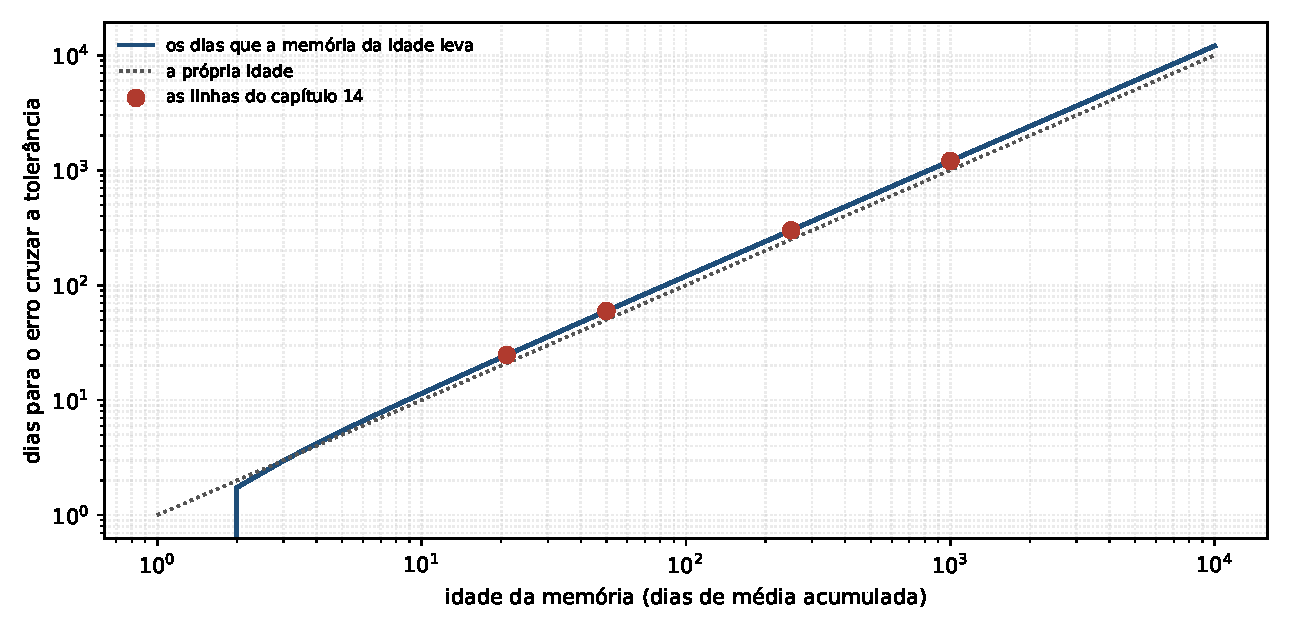
\includegraphics[width=\linewidth]{figuras/E26_aprender_1.pdf}
  \caption{Os dias que a memória da idade leva para cruzar a tolerância, contra a idade dela. Os
    dois eixos são logarítmicos; a linha pontilhada é a própria idade, e os pontos são as quatro
    linhas que o capítulo da memória já publicava. A curva e a reta são paralelas, e é isso que faz
    do caso um caso sem conserto.}
  \label{fig:idade}
\end{figure}

A distância entre a curva e a reta não cresce com a idade: ela fica em torno de vinte por cento em
toda a escala --- a razão vale \numAprenderRazaoVinteEUm{} aos vinte e um dias e
\numAprenderRazaoMil{} aos mil. Quem nunca esquece não fica cada vez mais para trás: fica sempre a
mesma fração atrás, e é por isso que esperar não resolve.

\section{O que custa escolher}

O conserto é o do capítulo da memória --- escolher a taxa em vez de herdar a idade ---, e o preço
dele se mede. Quatro estimadores, o mesmo degrau no dia \numConsertoQuando{}, o mesmo horizonte de
\numConsertoHorizonte{} dias e o mesmo mundo de \numConsertoDias{} dias: a média acumulada, a
exponencial de vinte e um dias, a acumulada que reinicia a cada \numConsertoJanela{} dias e a janela
de \numConsertoJanela{} dias.

\begin{table}[htbp]
  \centering
  \small
  \begin{tabular}{lr}
    \hline
    estimador & erro depois do degrau \\
    \hline
    a janela de \numConsertoJanela{} dias & \numConsertoErroJanela \\
    a exponencial de vinte e um dias & \numConsertoErroExponencial \\
    a média acumulada & \numConsertoErroAcumulada \\
    a acumulada que reinicia & \numConsertoErroReinicia \\
    \hline
  \end{tabular}
  \caption{O erro de cada estimador no mesmo horizonte, em \numConsertoMundos{} mundos. O degrau é o
    do capítulo da memória, e a tolerância daquele capítulo é de \numEsquecimentoTolerancia{} do
    nível novo.}
  \label{tab:conserto}
\end{table}

A ordem é a lição. \textbf{Escolher a memória corta o erro para menos da metade}: a pior das quatro
erra \numConsertoRazaoPiorMelhor{} vezes o que a melhor erra. E o conserto ingênuo não é conserto: a
acumulada que reinicia a cada janela erra \numConsertoErroReinicia, mais do que a que nunca esquece
--- uma média recém-nascida é tão cega quanto uma média velha é surda, e reiniciar só troca uma
cegueira pela outra.

\begin{figure}[htbp]
  \centering
  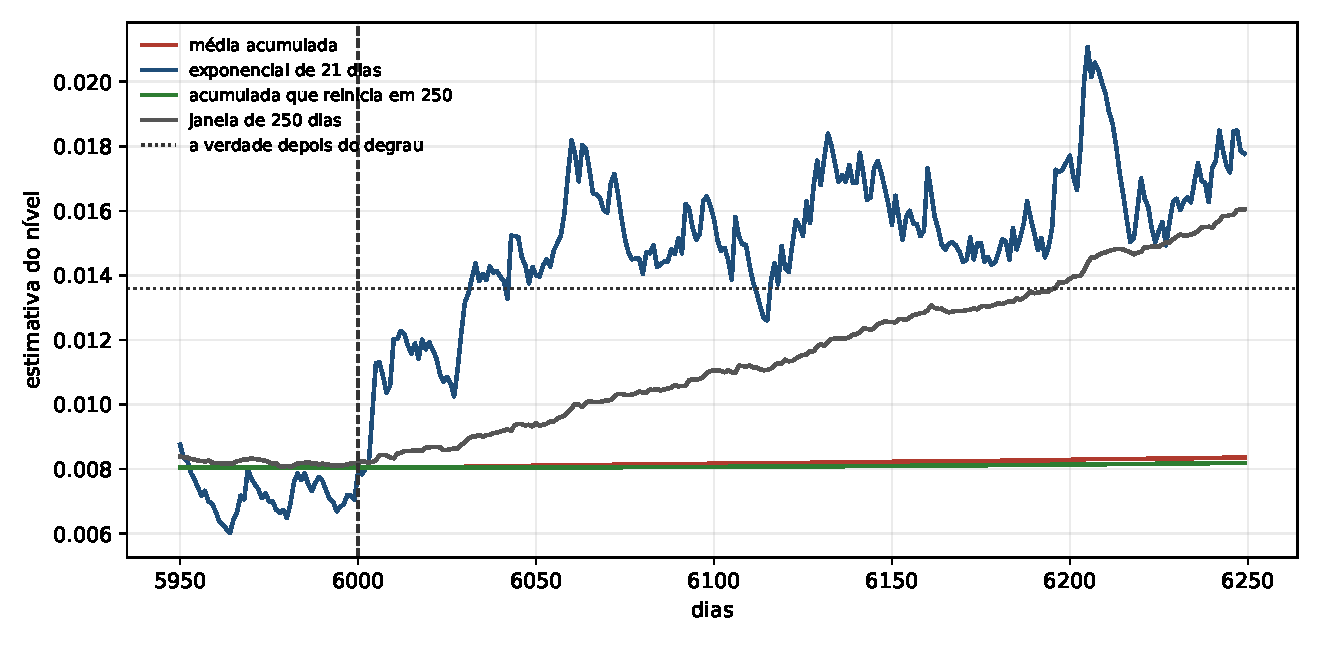
\includegraphics[width=\linewidth]{figuras/E27_conserto_1.pdf}
  \caption{Os quatro estimadores em torno do dia do degrau, contra a verdade. Depois dele a
    exponencial de vinte e um dias reage e oscila em volta da linha; a janela sobe em rampa, porque
    vai sendo preenchida por dias novos; e a média acumulada e a que reinicia ficam paradas --- elas
    carregam tanto passado que o degrau quase não as move dentro do horizonte da decisão.}
  \label{fig:conserto}
\end{figure}

\section{O que fica}

Fica a resposta, e ela é estreita: o estimador mais barato de escrever é o mais caro de usar. A
memória não é um resíduo da idade do sistema --- é uma escolha, e escolhê-la tem preço declarado,
medido no mesmo horizonte em que a decisão acontece.

O que sobra é o fracasso seguinte, e ele é do tamanho da escolha que se acabou de fazer. A taxa do
capítulo da memória foi medida num mundo que ou não muda ou dobra de uma vez, e a desta seção, no
mesmo mundo. \textbf{Escolher a memória exige saber quanto tempo o mundo fica parado} --- e esse
tempo não é um dado da série: é uma borda que quem decide declara. É o que o enquadramento vai
medir: onde a série começa e termina, de quando é o dado que chega, e quanto passado ainda conta.
